% Provenance (never printed): enseignement scientifique premiere (2019),
% "La Terre, un astre singulier" (the place of the Earth) and the old seconde
% SVT "La planete Terre, une planete habitable" (conditions for liquid water,
% the habitable zone); see sources/book2/PROVENANCE.md. Every temperature,
% phase boundary and habitable-zone limit is computed in
% figdata/grade-10/planet_temperatures.py.
\chapter{Planet yang Layak Huni}\label{ch:g10:habitable-planet}

Tiga planet batuan beredar berdampingan mengelilingi Matahari. Di permukaan
Venus, udaranya begitu rapat sehingga menekan sembilan puluh dua kali lebih
kuat daripada di Bumi, dan begitu panas --- lebih dari
\qty{460}{\degreeCelsius} --- sehingga timbal pun akan mencair. Di Mars, udara
yang tipis menekan kurang dari seperseratus tekanan udara kita, dan suhu
rata-ratanya jauh di bawah titik beku. Di antara keduanya, Bumi memiliki
samudra, hujan, dan kehidupan. Ketiga planet itu terbentuk dari piringan gas
dan debu yang sama di sekeliling Matahari muda, dari batuan yang hampir sama.
Mengapa nasibnya begitu berbeda? Bab ini membahas apa yang menentukan suhu
sebuah planet, apa yang membuatnya dapat mempertahankan atmosfer, dalam
kondisi apa air dapat berwujud cair, dan di mana, di sekitar Matahari dan di
sekitar bintang-bintang lain, kondisi seperti itu dapat ditemukan.
% ledger: nasa:venus-atm, nasa:mars-atm, planet:Venus.Tmean

\begin{omfigure}
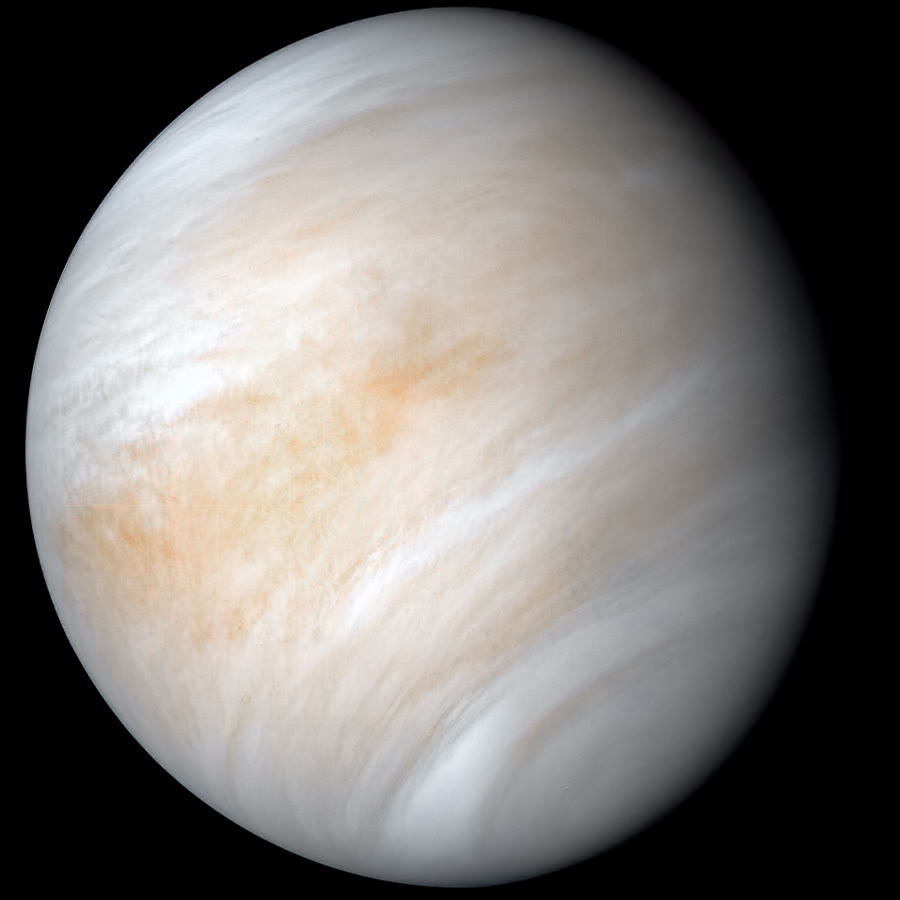
\includegraphics[width=0.38\linewidth]{images/book2/g10-nasa-venus-mariner10.jpg}

{\small Venus dilihat oleh wahana Mariner~10 pada 1974, dengan warna yang
mendekati apa yang akan dilihat mata: sebuah planet yang seluruhnya terbungkus
awan. Citra: NASA/JPL-Caltech (domain publik).}
\end{omfigure}

\begin{recall}
Matahari adalah sebuah bintang; di sekelilingnya beredar empat planet batuan,
yaitu Merkurius, Venus, Bumi, dan Mars, lalu empat planet raksasa, pada orbit
yang hampir berbentuk lingkaran (buku-buku fisika dan Buku 1). Setiap benda
memancarkan energi berupa cahaya, makin banyak seiring naiknya suhu, dan pada
suhu planet sebagian besar berupa cahaya inframerah (buku-buku fisika). Gas
rumah kaca --- uap air, karbon dioksida, metana --- menyerap sebagian
inframerah yang dipancarkan permukaan dan membuatnya tetap lebih hangat
(buku-buku kimia). Air terdapat sebagai es, air cair, dan uap air; tekanan
adalah gaya per satuan luas, yang diukur dalam pascal (buku-buku fisika).
\end{recall}

\section{Suhu yang ditentukan oleh bintang}

Matahari memancarkan cahayanya sama besar ke segala arah. Pada jarak $d$,
dayanya $L$ (\emph{luminositasnya}) tersebar pada bola seluas $4\pi d^2$.

\begin{proposition}[Hukum kuadrat terbalik cahaya Matahari]\label{prop:g10:habitable-planet:inverse-square}
Daya yang diterima per meter persegi yang menghadap Matahari, yaitu
\emph{iradiansi Matahari}, pada jarak $d$ dari Matahari adalah
\[
  S = \frac{L}{4\pi d^2}.
\]
Pada jarak Bumi, \qty{1}{au}, $S_0 = \qty{1361}{W/m^2}$; pada jarak $d$ yang
diukur dalam satuan astronomi, $S = S_0/d^2$.
\end{proposition}

\begin{proof}
Di ruang hampa tidak ada cahaya yang hilang, jadi seluruh daya $L$ melewati
setiap bola yang berpusat di Matahari; pada bola berjari-jari $d$ daya itu
terbagi pada $4\pi d^2$ meter persegi. Menggandakan $d$ melipatempatkan luas
itu dan membagi $S$ dengan empat.
\end{proof}
% ledger: earth:TSI, sun:L, const:au

\begin{omfigure}
\begin{tikzpicture}[font=\small, >={Stealth[length=2mm]}]
  \shade[ball color=yellow!70!orange] (0,0) circle (0.35);
  \node[below=4pt] at (0,-0.35) {Matahari};
  \draw[omThm!70, thick] (0,0) -- (3,0.6) (0,0) -- (3,-0.6);
  \draw[omThm!70, thick, dashed] (3,0.6) -- (6,1.2) (3,-0.6) -- (6,-1.2);
  \draw[fill=omDef!25, draw=omDef!80!black] (3,-0.6) rectangle (3.18,0.6);
  \draw[fill=omDef!12, draw=omDef!80!black] (6,-1.2) rectangle (6.18,1.2);
  \draw[omDef!80!black] (6,0) -- (6.18,0) (6.09,-1.2) -- (6.09,1.2);
  \node[anchor=north] at (3.1,-0.7) {$d$};
  \node[anchor=north] at (6.1,-1.3) {$2d$};
  \node[anchor=south east, align=right, font=\footnotesize] at (2.9,0.75) {1 persegi:\\seluruh cahaya};
  \node[anchor=west, align=left, font=\footnotesize] at (6.35,0.6) {4 persegi:\\masing-masing seperempat};
  \draw[->, black!60] (0.5,-1.95) -- (6.1,-1.95);
  \node[anchor=north, font=\footnotesize] at (3.3,-2.0) {jarak dari Matahari};
\end{tikzpicture}

{\small Cahaya yang melewati satu persegi pada jarak $d$ tersebar pada empat
persegi yang sama besar pada jarak $2d$: iradiansi berkurang sebanding dengan
kebalikan kuadrat jarak.}
\end{omfigure}

Sebuah planet menyerap bagian cahaya ini yang tidak dipantulkannya, dan
memancarkan energi ke angkasa sebagai cahaya inframerah. Jika planet menyerap
lebih banyak daripada yang dipancarkannya, planet itu menghangat; makin hangat,
makin banyak yang dipancarkannya; akhirnya suhunya mantap pada nilai saat
keduanya seimbang.

\begin{definition}[Suhu kesetimbangan]\label{def:g10:habitable-planet:equilibrium-temperature}
Yang disebut \emph{suhu kesetimbangan}\index{suhu kesetimbangan} sebuah
planet adalah suhu ketika sebuah benda yang memancar seperti pemancar sempurna
akan mengirim ke angkasa daya yang tepat sama dengan daya yang diserap planet
itu dari bintangnya. Bagian cahaya datang yang dipantulkan planet secara
keseluruhan adalah \emph{albedo Bond}-nya, $A$.
\end{definition}

\begin{proposition}[Menghitung suhu kesetimbangan]\label{prop:g10:habitable-planet:teq}
Untuk planet yang menyebarkan kalor yang diserapnya ke seluruh permukaannya,
\[
  T_{\mathrm{eq}} = \left(\frac{S\,(1-A)}{4\sigma}\right)^{1/4},
  \qquad \sigma = \qty{5.67e-8}{W.m^{-2}.K^{-4}}.
\]
Pada jarak Bumi dan tanpa pemantulan sama sekali, rumus ini memberikan
\qty{278.3}{K}; pada jarak $d$ dalam satuan astronomi dan dengan albedo $A$,
$T_{\mathrm{eq}} = \qty{278.3}{K} \times (1-A)^{1/4}/\sqrt{d}$.
\end{proposition}

\begin{proof}[Bukti sebagian]
Planet itu menangkap cahaya Matahari pada sebuah piringan seluas $\pi R^2$
dan menyerap daya $(1-A)\,S\,\pi R^2$. Planet itu memancar dari seluruh
permukaannya, $4\pi R^2$. Pemancar sempurna bersuhu $T$ memancarkan
$\sigma T^4$ per meter persegi (hukum yang dibuktikan di buku-buku fisika,
diterima di sini). Menyamakan $4\pi R^2 \sigma T^4 = (1-A)\,S\,\pi R^2$
memberikan rumusnya; jari-jarinya saling menghapus. Dengan $S = S_0/d^2$,
akar pangkat empat dari $1/d^2$ adalah $1/\sqrt d$.
\end{proof}
% ledger: const:sigma, earth:TSI

\begin{example}[Bumi]\label{ex:g10:habitable-planet:earth}
% ledger: earth:TSI, earth:albedo, earth:Tbb, earth:Tsurf
Dengan $S_0 = \qty{1361}{W/m^2}$ dan $A = 0.294$,
$T_{\mathrm{eq}} = 278.3 \times 0.706^{1/4} \approx \qty{255}{K}$, yaitu
\qty{-18}{\degreeCelsius}. (Lembar fakta NASA mencantumkan \qty{254}{K}.) Suhu
rata-rata permukaan Bumi adalah \qty{288}{K}, \qty{15}{\degreeCelsius}: efek
rumah kaca atmosfer menghangatkannya sekitar \qty{33}{K}. Tanpa efek itu,
samudra akan membeku.
\end{example}

\begin{omfigure}
\begin{tikzpicture}
\begin{axis}[ybar, width=0.86\linewidth, height=5.8cm, ymin=0, ymax=950,
  bar width=10pt, enlarge x limits=0.15, symbolic x coords={Mercury,Venus,Earth,Moon,Mars},
  xtick=data, xticklabels={Merkurius,Venus,Bumi,Bulan,Mars}, ylabel={suhu (K)}, ymajorgrids, grid style={gray!22},
  legend style={at={(0.97,0.95)}, anchor=north east, font=\footnotesize, draw=black!30},
  nodes near coords, nodes near coords style={font=\scriptsize, rotate=90, anchor=west, /pgf/number format/fixed, /pgf/number format/precision=0},
  tick label style={font=\small}, label style={font=\small}]
\addplot[fill=omDef!45, draw=omDef!80!black] table[x=name, y=Teq_K] {figdata/out/grade-10-planet_temperatures-planets.dat};
\addlegendentry{suhu kesetimbangan}
\addplot[fill=omThm!55, draw=omThm!80!black] table[x=name, y=Tmean_K] {figdata/out/grade-10-planet_temperatures-planets.dat};
\addlegendentry{suhu permukaan rata-rata terukur}
\end{axis}
\end{tikzpicture}

{\small \omterm{def:g10:habitable-planet:equilibrium-temperature}{Suhu kesetimbangan} yang dihitung dari jarak dan albedo Bond setiap
benda, di samping suhu rata-rata permukaannya yang terukur. Data: lembar fakta
planet NASA.}
\end{omfigure}

\begin{remark}[Membaca diagram]\label{rem:g10:habitable-planet:reading}
% ledger: nasa:bond-albedos, planet:Mercury.Tmean, planet:Venus.Tmean, planet:Moon.Tmean, planet:Mars.Tmean, planet:Moon.day, nasa:moon-temps
Untuk Merkurius dan Mars, yang hampir tidak beratmosfer atau atmosfernya
sangat tipis, rata-rata terukur mendekati \omterm{def:g10:habitable-planet:equilibrium-temperature}{suhu kesetimbangan}. Rata-rata Bulan
berada di bawahnya: siang dan malamnya masing-masing berlangsung sekitar dua
minggu, dan permukaannya berayun dari sekitar \qty{95}{K} sampai \qty{390}{K},
sesuatu yang tidak tertangkap oleh rumus sederhana yang dibuat untuk planet
yang menyebarkan kalornya secara merata. Venus adalah kasus yang mencolok:
dengan albedo Bond 0.77 --- awannya memantulkan sebagian besar cahaya Matahari
--- \omterm{def:g10:habitable-planet:equilibrium-temperature}{suhu kesetimbangannya} lebih rendah daripada \omterm{def:g10:habitable-planet:equilibrium-temperature}{suhu kesetimbangan} Bumi,
tetapi permukaannya lebih dari \qty{500}{K} lebih panas daripada itu: itulah
efek rumah kaca atmosfer karbon dioksidanya yang tebal.
\end{remark}

\section{Mempertahankan atmosfer}

Gas terdiri atas molekul-molekul yang terus bergerak, makin cepat bila gas
makin panas. Molekul di puncak atmosfer yang bergerak ke atas lebih cepat
daripada laju lepas planet --- laju yang diperlukan untuk meninggalkan
gravitasinya untuk selamanya (buku-buku fisika) --- hilang ke angkasa. Selama
miliaran tahun, planet kecil yang gravitasinya lemah kehilangan udaranya,
sedangkan planet besar mempertahankannya.

\begin{center}
\small
% ledger: planet:Mercury.vesc, planet:Venus.vesc, planet:Earth.vesc, planet:Moon.vesc, planet:Mars.vesc, planet:Mercury.psurf, planet:Venus.psurf, planet:Earth.psurf, planet:Moon.psurf, nasa:mars-atm
\begin{tabular}{lccc}
\hline
benda & laju lepas (\unit{km/s}) & tekanan permukaan (bar) & atmosfer \\
\hline
Bulan & 2.4 & 0 & tidak ada \\
Merkurius & 4.3 & 0 & tidak ada \\
Mars & 5.0 & 0.006 & tipis, karbon dioksida \\
Venus & 10.4 & 92 & tebal, karbon dioksida \\
Bumi & 11.2 & 1 & nitrogen dan oksigen \\
\hline
\end{tabular}
\end{center}

\begin{remark}[Ukuran bukan satu-satunya faktor]\label{rem:g10:habitable-planet:size}
Bulan dan Merkurius, yang kecil dan (untuk Merkurius) dekat dengan Matahari
yang panas, telah kehilangan hampir semua gasnya. Mars, dengan laju lepas
setengah laju lepas Bumi, mempertahankan atmosfer yang tipis. Venus dan Bumi
hampir sama ukuran dan laju lepasnya, tetapi atmosfernya sangat berbeda:
sejarahnya --- nasib air dan karbon dioksidanya --- berpisah jalan, seperti
akan ditunjukkan \cref{ch:g12:early-earth} untuk Bumi.
\end{remark}

\section{Air cair}

\begin{omfigure}
\begin{tikzpicture}
\begin{axis}[omrecord, width=0.88\linewidth, height=7.2cm, xmin=150, xmax=800,
  ymode=log, ymin=1e-6, ymax=2000, xlabel={suhu (K)}, ylabel={tekanan (bar)},
  xtick={200,300,...,800}, ytick={1e-6,1e-4,1e-2,1,100},
  log basis y=10]
\addplot[omDef!85!black, line width=1.1pt] table[x=T_K, y=p_bar] {figdata/out/grade-10-planet_temperatures-vap.dat};
\addplot[omDef!85!black, line width=1.1pt] table[x=T_K, y=p_bar] {figdata/out/grade-10-planet_temperatures-subl.dat};
\addplot[omDef!85!black, line width=1.1pt] table[x=T_K, y=p_bar] {figdata/out/grade-10-planet_temperatures-melt.dat};
\addplot[only marks, mark=*, mark size=2pt, black] coordinates {(273.16,0.00611657) (647.096,220.64)};
\addplot[only marks, mark=square*, mark size=2.4pt, omThm!85!black] table[x=T_K, y=p_bar] {figdata/out/grade-10-planet_temperatures-points.dat};
\node[font=\small] at (axis cs:205,30) {es};
\node[font=\small] at (axis cs:420,30) {cair};
\node[font=\small] at (axis cs:600,1e-3) {uap air};
\node[font=\footnotesize, anchor=north west] at (axis cs:276,0.0055) {titik tripel};
\node[font=\footnotesize, anchor=south east] at (axis cs:640,300) {titik kritis};
\node[font=\footnotesize, anchor=south, omThm!85!black] at (axis cs:737,110) {Venus};
\node[font=\footnotesize, anchor=west, omThm!85!black] at (axis cs:296,1.0) {Bumi};
\node[font=\footnotesize, anchor=north, omThm!85!black] at (axis cs:210,0.0045) {Mars};
\end{axis}
\end{tikzpicture}

{\small Diagram fase air, dengan kondisi rata-rata permukaan Venus, Bumi, dan
Mars (persegi). Sumbu tekanan berskala logaritmik: setiap tanda skala seratus
kali tanda di bawahnya. Kurva dihitung dari persamaan-persamaan Asosiasi
Internasional untuk Sifat-Sifat Air dan Uap (IAPWS); nilai-nilai planet dari
NASA.}
\end{omfigure}

\begin{proposition}[Kapan air dapat berwujud cair]\label{prop:g10:habitable-planet:liquid}
% ledger: iapws:triple-critical, iapws:vapour-pressure, iapws:melt-subl
Air cair hanya ada pada tekanan di atas tekanan \emph{titik tripel},
\qty{611.657}{Pa} (\qty{0.006}{bar}), tempat es, air cair, dan uap air
berdampingan pada \qty{273.16}{K}, dan pada suhu di bawah \emph{titik kritis},
\qty{647.096}{K} (\qty{220.64}{bar}), yang di atasnya air cair dan uap air
tidak dapat dibedakan lagi. Pada tekanan tertentu di atas titik tripel, air
berwujud cair di antara titik lelehnya, dekat \qty{273}{K}, dan titik
didihnya, yang turun bila tekanan turun.
\end{proposition}

\begin{example}[Tiga planet pada satu diagram]\label{ex:g10:habitable-planet:three}
% ledger: nasa:venus-atm, nasa:mars-atm, earth:psurf, earth:Tsurf (boiling point at 636 Pa computed)
Permukaan Bumi, pada \qty{288}{K} dan \qty{1}{bar}, berada di dalam daerah
cair: air di sana dapat berupa air cair, es, atau uap, bergantung pada cuaca.
Venus, pada \qty{737}{K}, berada jauh di atas suhu kritis: air cair sama
sekali tidak mungkin ada. Mars, pada \qty{6.36}{mbar}, berada sedikit di atas
titik tripel: air di sana mendidih pada sekitar \qty{0.5}{\degreeCelsius},
jadi air cair hanya dapat bertahan dalam rentang sekitar setengah derajat,
sedangkan suhu rata-ratanya, \qty{210}{K}, berada di daerah es.
\end{example}

\begin{omfigure}
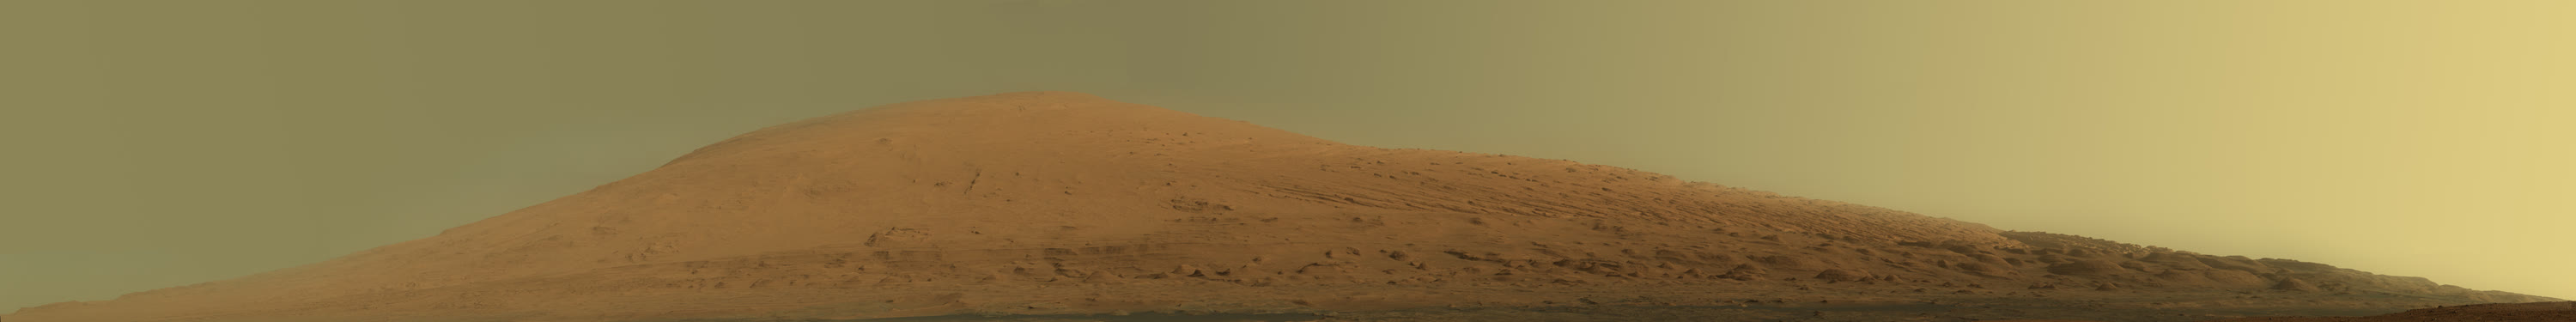
\includegraphics[width=0.96\linewidth]{images/book2/g10-nasa-mars-mount-sharp.jpg}

{\small Gunung Sharp, di dalam Kawah Gale di Mars, dipotret oleh wahana
penjelajah Curiosity pada 2012, dengan warna yang direkam kameranya.
Lapisan-lapisan bawahnya diendapkan di dalam air, miliaran tahun yang lalu.
Citra: NASA/JPL-Caltech/MSSS (domain publik).}
\end{omfigure}

\section{Zona layak huni}

\begin{definition}[Zona layak huni]\label{def:g10:habitable-planet:habitable-zone}
Yang disebut \emph{zona layak huni}\index{zona layak huni} sebuah bintang
adalah rentang jarak dari bintang itu tempat sebuah planet batuan yang
memiliki cukup air dan atmosfer seperti atmosfer Bumi dapat mempertahankan
air cair di permukaannya. Tepi dalamnya adalah tempat planet itu akan
kehilangan airnya karena panas; tepi luarnya adalah tempat efek rumah kaca
yang kuat pun tidak lagi dapat mencegah air itu membeku.
\end{definition}

\begin{proposition}[Zona layak huni Matahari]\label{prop:g10:habitable-planet:hz-sun}
% ledger: kopparapu:hz-sun, planet:Mercury.dist, planet:Venus.dist, planet:Mars.dist
Model-model rinci atmosfer planet menempatkan \omterm{def:g10:habitable-planet:habitable-zone}{zona layak huni} Matahari di
antara \qty{0.99}{au} dan \qty{1.70}{au}. Bumi (\qty{1}{au}) berada sedikit
di sebelah dalam tepi dalamnya; Mars (\qty{1.52}{au}) berada di dalam zona
itu; Venus (\qty{0.72}{au}) berada jauh di sebelah dalam tepi dalamnya.
\end{proposition}

\begin{proposition}[Zona layak huni bintang-bintang lain]\label{prop:g10:habitable-planet:hz-scaling}
Di sekitar bintang berluminositas $L$, sebuah planet menerima iradiansi yang
sama dengan pada jarak $d_\odot$ dari Matahari bila planet itu terletak pada
\[
  d = d_\odot \sqrt{L/L_\odot}.
\]
Tepi-tepi \omterm{def:g10:habitable-planet:habitable-zone}{zona layak huni} bergeser dengan perbandingan yang sama, dalam
pendekatan pertama (warna cahaya bintang juga sedikit berpengaruh).
\end{proposition}

\begin{proof}
Iradiansi yang sama berarti $L/(4\pi d^2) = L_\odot/(4\pi d_\odot^2)$, jadi
$d^2 = d_\odot^2\,L/L_\odot$.
\end{proof}

\begin{omfigure}
\begin{tikzpicture}[font=\small]
  % top: the Sun, 0-2 au over 12 cm (6 cm per au)
  \fill[omProp!30] (0.99*6,0) rectangle (1.70*6,0.5);
  \draw[black!70] (0,0.25) -- (12.3,0.25);
  \foreach \x in {0,0.5,...,2} \draw (\x*6,0.15) -- (\x*6,0.35) node[pos=0, below=1pt, font=\footnotesize] {\x};
  \shade[ball color=yellow!70!orange] (0,0.25) circle (0.22);
  \foreach \n/\d in {Merkurius/0.387, Venus/0.723, Bumi/1.0, Mars/1.524} {
    \fill[omThm!85!black] (\d*6,0.25) circle (2.2pt);
    \node[anchor=south, font=\footnotesize] at (\d*6,0.55) {\n};
  }
  \node[anchor=west, font=\footnotesize] at (12.4,0.25) {au};
  \node[anchor=north, font=\footnotesize] at (8.07,-0.25) {zona layak huni, 0.99--1.70 au};
  \node[anchor=east, font=\footnotesize] at (-0.3,0.25) {Matahari};
  % bottom: Proxima Centauri, 0-0.1 au over 12 cm (120 cm per au)
  \begin{scope}[yshift=-2.2cm]
  \fill[omProp!30] (0.0385*120,0) rectangle (0.0661*120,0.5);
  \draw[black!70] (0,0.25) -- (12.3,0.25);
  \foreach \x/\l in {0/0, 0.025/0.025, 0.05/0.05, 0.075/0.075, 0.1/0.1} \draw (\x*120,0.15) -- (\x*120,0.35) node[pos=0, below=1pt, font=\footnotesize] {\l};
  \shade[ball color=red!70!orange] (0,0.25) circle (0.14);
  \fill[omThm!85!black] (0.0485*120,0.25) circle (2.2pt);
  \node[anchor=south, font=\footnotesize] at (0.0485*120,0.55) {Proxima b};
  \node[anchor=west, font=\footnotesize] at (12.4,0.25) {au};
  \node[anchor=north, font=\footnotesize] at (6.28,-0.25) {zona layak huni, 0.038--0.066 au};
  \node[anchor=east, align=right, font=\footnotesize] at (-0.3,0.25) {Proxima\\Centauri};
  \end{scope}
\end{tikzpicture}

{\small Atas: \omterm{def:g10:habitable-planet:habitable-zone}{zona layak huni} Matahari dan keempat planet batuan. Bawah: \omterm{def:g10:habitable-planet:habitable-zone}{zona
layak huni} bintang merah redup Proxima Centauri, yang dihitung dengan
menskalakan zona Matahari dengan akar kuadrat luminositas bintang itu, beserta
planetnya, Proxima~b. Perhatikan perubahan skalanya: seluruh jalur bawah
panjangnya hanya \qty{0.1}{au}.}
\end{omfigure}

\section{Planet-planet bintang lain}

\begin{definition}[Eksoplanet]\label{def:g10:habitable-planet:exoplanet}
Yang disebut \emph{eksoplanet}\index{eksoplanet} adalah planet yang
mengorbit bintang selain Matahari.
\end{definition}

\omterm{def:g10:habitable-planet:exoplanet}{Eksoplanet} terlalu redup dan terlalu dekat dengan bintangnya untuk dapat
dilihat secara langsung, kecuali beberapa planet raksasa. Sebagian besar
ditemukan secara tidak langsung: planet itu melintas di depan bintangnya sekali
setiap orbit dan meredupkannya sedikit sekali, atau tarikannya membuat bintang
itu bergoyang mendekat dan menjauhi kita, sehingga warna cahaya bintang itu
bergeser bolak-balik. Metode kedua hanya memberikan massa \emph{minimum}
planet, karena kemiringan orbitnya tidak diketahui. Metode-metode ini
dipelajari dalam jilid Sarjana Tahun ke-3.

\begin{dated}{2026}
% ledger: nea:count-2026
Pada 15 Oktober 2026, NASA Exoplanet Archive mencatat 6\,451 \omterm{def:g10:habitable-planet:exoplanet}{eksoplanet} yang
telah dikonfirmasi.
\end{dated}

\begin{example}[Proxima b]\label{ex:g10:habitable-planet:proxima}
% ledger: nea:proxima-b (flux and habitable zone computed in figdata/grade-10/planet_temperatures.py)
Bintang terdekat dari Matahari, Proxima Centauri, yang berjarak
\qty{1.30}{\parsec}, adalah bintang merah kecil yang luminositasnya hanya
sekitar $0.0015$ luminositas Matahari. Pada 2016 ditemukan sebuah planet yang
mengorbitnya setiap 11.2 hari, pada \qty{0.0485}{au}, dengan massa
sekurang-kurangnya 1.06 kali massa Bumi. Pada jarak itu planet tersebut
menerima sekitar 0.64 iradiansi yang diterima Bumi, dan planet itu terletak di
dalam \omterm{def:g10:habitable-planet:habitable-zone}{zona layak huni} bintangnya. Apakah planet itu memiliki atmosfer, atau
air, belum diketahui.
\end{example}

\begin{remark}[Layak huni bukan berarti berpenghuni]\label{rem:g10:habitable-planet:inhabited}
\omterm{def:g10:habitable-planet:habitable-zone}{Zona layak huni} hanyalah pernyataan tentang jarak dan cahaya. Planet di
dalamnya mungkin tidak memiliki air, tidak memiliki atmosfer, atau memiliki
atmosfer yang keliru --- Mars terletak di dalam zona Matahari dan saat ini
tidak memiliki air cair di permukaannya. Bumi layak huni karena beberapa
syarat terpenuhi sekaligus: jarak yang tepat, massa yang cukup besar untuk
mempertahankan atmosfer, air yang melimpah, dan efek rumah kaca yang tidak
terlalu lemah ataupun terlalu kuat.
\end{remark}

\section{Latihan}

\begin{exercise}[$\star$]\label{exo:g10:habitable-planet:1}
Definisikan \omterm{def:g10:habitable-planet:equilibrium-temperature}{suhu kesetimbangan} sebuah planet. Mengapa suhu rata-rata permukaan
Bumi lebih tinggi daripada \omterm{def:g10:habitable-planet:equilibrium-temperature}{suhu kesetimbangannya}?
\end{exercise}

\begin{exercise}[$\star$]\label{exo:g10:habitable-planet:2}
Dengan diagram batang \omterm{def:g10:habitable-planet:equilibrium-temperature}{suhu kesetimbangan} dan suhu terukur, sebutkan benda yang
permukaannya paling banyak dihangatkan oleh atmosfernya, dan perkirakan
berapa kelvin.
\end{exercise}

\begin{exercise}[$\star$]\label{exo:g10:habitable-planet:3}
Mars mengorbit pada jarak \qty{1.52}{au} dari Matahari. Dengan hukum kuadrat
terbalik dan $S_0 = \qty{1361}{W/m^2}$, hitung iradiansi Matahari di Mars.
\end{exercise}

\begin{exercise}[$\star$]\label{exo:g10:habitable-planet:4}
Dengan diagram fase air, tentukan wujud air pada \qty{1}{bar} dan
\qty{330}{K}; pada \qty{0.001}{bar} dan \qty{250}{K}; pada \qty{100}{bar} dan
\qty{700}{K}.
\end{exercise}

\begin{exercise}[$\star$]\label{exo:g10:habitable-planet:5}
Apa itu \omterm{def:g10:habitable-planet:exoplanet}{eksoplanet}? Uraikan, masing-masing dalam satu kalimat, dua cara utama
untuk mendeteksi \omterm{def:g10:habitable-planet:exoplanet}{eksoplanet}.
\end{exercise}

\begin{exercise}[$\star\star$]\label{exo:g10:habitable-planet:6}
Hitung \omterm{def:g10:habitable-planet:equilibrium-temperature}{suhu kesetimbangan} Bumi dengan $S_0 = \qty{1361}{W/m^2}$ dan
$A = 0.294$, lalu dengan $A = 0$. Ubah keduanya ke derajat Celsius.
\end{exercise}

\begin{exercise}[$\star\star$]\label{exo:g10:habitable-planet:7}
Sebuah bintang empat kali lebih terang daripada Matahari. Di antara jarak
berapa \omterm{def:g10:habitable-planet:habitable-zone}{zona layak huninya} berada? Apakah Bumi, bila ditempatkan pada jarak
\qty{1}{au} darinya, berada di dalamnya?
\end{exercise}

\begin{exercise}[$\star\star$]\label{exo:g10:habitable-planet:8}
Venus mengorbit pada jarak \qty{0.723}{au}. Hitung iradiansi yang diterimanya,
lalu \omterm{def:g10:habitable-planet:equilibrium-temperature}{suhu kesetimbangannya} dengan albedo Bond 0.77. Bandingkan dengan suhu
permukaannya, \qty{737}{K}, dan jelaskan perbedaannya.
\end{exercise}

\begin{exercise}[$\star\star$]\label{exo:g10:habitable-planet:9}
Di Mars tekanan permukaan rata-rata adalah \qty{6.36}{mbar}, sedikit di atas
titik tripel air, dan air di sana mendidih pada sekitar
\qty{0.5}{\degreeCelsius}. Jelaskan mengapa air cair tidak dapat bertahan di
permukaan Mars saat ini, bahkan pada sore musim panas ketika tanahnya mencapai
\qty{10}{\degreeCelsius}.
\end{exercise}

\begin{exercise}[$\star\star$]\label{exo:g10:habitable-planet:10}
Laju lepas di Bulan \qty{2.4}{km/s} dan di Bumi \qty{11.2}{km/s}. Hitung
perbandingannya. Jelaskan mengapa Bumi dapat mempertahankan atmosfer
sedangkan Bulan tidak.
\end{exercise}

\begin{exercise}[$\star\star$]\label{exo:g10:habitable-planet:11}
Andaikan Bumi tertutup es dan albedo Bond-nya naik menjadi 0.50. Hitung \omterm{def:g10:habitable-planet:equilibrium-temperature}{suhu
kesetimbangannya} yang baru. Jelaskan mengapa keadaan seperti itu, sekali
tercapai, cenderung bertahan.
\end{exercise}

\begin{exercise}[$\star\star\star$]\label{exo:g10:habitable-planet:12}
Tunjukkan bahwa $T_{\mathrm{eq}} = \qty{278.3}{K} \times (1-A)^{1/4}/\sqrt{d}$,
dengan $d$ dalam satuan astronomi, diturunkan dari rumus dalam bab ini.
Dengan faktor berapa \omterm{def:g10:habitable-planet:equilibrium-temperature}{suhu kesetimbangan} berubah bila jaraknya dikalikan empat?
\end{exercise}

\begin{exercise}[$\star\star\star$]\label{exo:g10:habitable-planet:13}
Pada jarak berapa dari Matahari sebuah planet beralbedo 0.294 akan memiliki
\omterm{def:g10:habitable-planet:equilibrium-temperature}{suhu kesetimbangan} \qty{273}{K}? Bandingkan dengan tepi dalam \omterm{def:g10:habitable-planet:habitable-zone}{zona layak huni},
dan jelaskan mengapa keduanya berbeda.
\end{exercise}

\begin{exercise}[$\star\star\star$]\label{exo:g10:habitable-planet:14}
Di sebuah planet yang tekanan permukaannya \qty{1000}{Pa}, air mendidih pada
sekitar \qty{7}{\degreeCelsius}. Di antara suhu berapa air dapat berwujud cair
di sana? Apa yang akan terjadi pada sebuah danau di planet itu pada hari yang
bersuhu \qty{15}{\degreeCelsius}?
\end{exercise}

\begin{exercise}[$\star\star\star$]\label{exo:g10:habitable-planet:15}
Sebuah planet mengorbit pada jarak \qty{1.2}{au} dari bintang yang luminositasnya
setengah luminositas Matahari. Hitung tepi-tepi \omterm{def:g10:habitable-planet:habitable-zone}{zona layak huni} bintang itu dan
tentukan apakah planet itu berada di dalamnya. Seberapa yakin kita dapat
menjawabnya?
\end{exercise}

\section{Soal: Dapatkah Proxima b Menyimpan Samudra?}

\begin{problem}[{Soal akhir pekan --- dari cahaya sebuah bintang merah redup
sampai suhu planet terdekatnya}]
\label{pb:g10:habitable-planet:1}
% ledger: nea:proxima-b, kopparapu:hz-sun, earth:TSI, earth:albedo, planet:Earth.vesc, nasa:bond-albedos (all results computed in figdata/grade-10/planet_temperatures.py or from the rounded data below)
Seorang siswa membaca lembar data planet Proxima~b. Bintangnya memiliki
luminositas $L = 0.00151\,L_\odot$; planet itu mengorbit pada
$d = \qty{0.0485}{au}$ dalam 11.18 hari dan memiliki massa
sekurang-kurangnya 1.055 kali massa Bumi. Gunakan
$S_0 = \qty{1361}{W/m^2}$, $\sigma = \qty{5.67e-8}{W.m^{-2}.K^{-4}}$, \omterm{def:g10:habitable-planet:habitable-zone}{zona
layak huni} Matahari \qtyrange{0.99}{1.70}{au}, dan laju lepas Bumi
\qty{11.2}{km/s}.

\medskip
\noindent\textbf{Bagian I --- Cahaya bintang.}
\begin{enumerate}
  \item Hitung iradiansi di planet itu sebagai bagian dari iradiansi di Bumi,
        $L/d^2$ (dengan $L$ dalam luminositas Matahari dan $d$ dalam au).
  \item Nyatakan iradiansi itu dalam \unit{W/m^2}.
  \item Bandingkan dengan iradiansi di Venus (\qty{2601}{W/m^2}) dan di
        Mars (\qty{586}{W/m^2}).
  \item Berapa tahun planet itu termuat dalam satu tahun Bumi?
\end{enumerate}

\medskip
\noindent\textbf{Bagian II --- Suhu tanpa atmosfer.}
\begin{enumerate}[resume]
  \item Hitung \omterm{def:g10:habitable-planet:equilibrium-temperature}{suhu kesetimbangan} sebuah planet yang hitam sempurna
        ($A = 0$) pada iradiansi itu.
  \item Hitung suhu itu untuk planet yang seterang Venus ($A = 0.77$).
  \item Manakah di antara kedua suhu itu yang berada di atas titik beku air?
        Apa yang ditunjukkan kedua hasil itu tentang peran awan dan
        es?
\end{enumerate}

\medskip
\noindent\textbf{Bagian III --- Zona layak huni.}
\begin{enumerate}[resume]
  \item Hitung $\sqrt{L/L_\odot}$.
  \item Hitung tepi dalam \omterm{def:g10:habitable-planet:habitable-zone}{zona layak huni} bintang itu.
  \item Hitung tepi luarnya.
  \item Apakah Proxima~b berada di dalam \omterm{def:g10:habitable-planet:habitable-zone}{zona layak huni}?
  \item Pada jarak berapa dari Matahari sebuah planet akan menerima iradiansi
        yang sama dengan Proxima~b? Di bagian mana \omterm{def:g10:habitable-planet:habitable-zone}{zona layak huni} Matahari
        tempat itu berada?
\end{enumerate}

\medskip
\noindent\textbf{Bagian IV --- Atmosfer dan air?}
\begin{enumerate}[resume]
  \item Jika planet itu memiliki massa jenis rata-rata Bumi, jari-jarinya
        akan $1.055^{1/3}$ kali jari-jari Bumi. Hitung faktor ini.
  \item Laju lepas sebanding dengan $\sqrt{M/R}$. Perkirakan laju lepas
        planet itu. Dapatkah planet itu mempertahankan atmosfer?
  \item Mengapa massanya hanya diketahui sebagai nilai minimum?
  \item Pada diagram fase, berapa tekanan permukaan terendah yang masih
        memungkinkan adanya air cair?
  \item Hitung \omterm{def:g10:habitable-planet:equilibrium-temperature}{suhu kesetimbangan} Proxima~b dengan albedo Bumi, 0.294.
  \item Berapa kelvin efek rumah kacanya kemudian harus menghangatkan planet
        itu agar permukaannya mencapai suhu rata-rata Bumi,
        \qty{288}{K}?
\end{enumerate}
\end{problem}
